% Chapter 3

\chapter{Category Theory and Lattice Models} % Main chapter title

\label{Chapter3} % For referencing the chapter elsewhere, use \ref{Chapter3} 

\lhead{Chapter 3. \emph{Category Theory and Lattice Models}} % This is for the header on each page - perhaps a shortened title

%----------------------------------------------------------------------------------------

\section{Levin-Wen Models}
    The aim of this section is to introduce the most general structure used to classify topological phases of matter. This uses the concepts presented in Chapter
\ref{Chapter1} and it will be shown that the contents presented in Chapter \ref{Chapter2} will form a subclass of these models in Chapter \ref{Chapter4}. The String Net Model
or Levin-Wen Model \citep{Reference3} is defined on trivalent graph embedded to a closed oriented surface. The rules of the model are as follows : \\

\begin{itemize}
\item[1] String types : They are finite number of string types, and the set of string types is isomorphic to positive integers.\\
\item[2] Branching rules : Only certain string types are allowed to form a  vertex.\\
\item[3] String orientation : Every string has a dual type, which is directed in the opposite direction.
\end{itemize}

The universal features of the string net model are given by fig \ref{fig:Levin_Wen_features} :
\begin{figure}
  \centering
      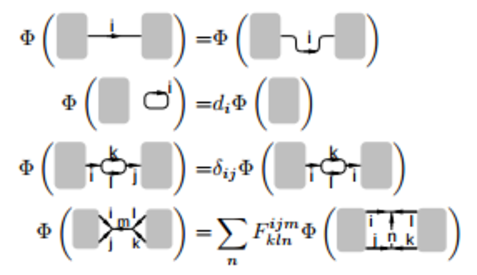
\includegraphics[width=8cm]{Levin_Wen_conditions.pdf}
      \caption[Features of Levin-Wen Model]{Universal features of the String-Net Model}
  \centering    
  \label{fig:Levin_Wen_features}
\end{figure}

Equivalently, they are captured by six index object $F_{ijk}^{klm}$ and the numbers $d_{i}$, that is the $F$ moves and the quantum dimensions. However not
all combinations of these give rise to string net model as they are constrainted by the above equations. The only valid combinations are those
which satisfy :
\begin{center}
$F^{ijk}_{j^{*}i^{*}0} = \frac{\sqrt{d_{k}}}{\sqrt{d_{i}d_{k}}}\delta_{ijk}$ \\
$F^{ijm}_{kln} = F^{klm^{*}}_{jin} = F^{jim}_{lkn^{*}} = F^{imj}_{k^{*}ln}\frac{\sqrt{d_{m}d_{n}}}{\sqrt{d_{j}d_{l}}}$ \\
$\varSigma_{n=0}^{N}F^{mlq}_{kp^{*}n}F^{jip}_{mns^{*}}F^{js^{*}n}_{lkr^{*}} = F^{jip}_{q^{*}kr^{*}}F^{riq^{*}}_{mls^{*}}$ 
\end{center}

Unitary Tensor Categories are the fundamental framework for the string net model. The string labels form the objects in category,
the Homspace can be seen as branching rules. Given a group $G$, the string labels are the irreducible representations of the group
$G$, the quantum dimension $d_{i}$ is the dimension of the representation, and the $F$ object is the $6j$ symbols of the group.

For every valid  $(F^{ijk}_{lmn}, d_{i})$,  the Hamiltonian of the model is given by :
\begin{center}
 $H = -\sum_{I}Q_{I} - \sum_{p}B_{p}$, where  $B_{p} = \sum_{s=0}^{N}a_{s}B_{p}^{s}$
\end{center}
where $Q_{I}$ measures the electric charge and favors no charge configuration, and $B_{p}$ measures the magnetic flux through a plaquette
and favors no flux. The figure \ref{fig:QvBp_Levin_Wen} give the action of $Q_{I}$ and $B_{\bold{p}}$ on a arbitrary lattice.
\begin{figure}
\centering

\includegraphics[width=9cm]{Q_I_LW.pdf}\\
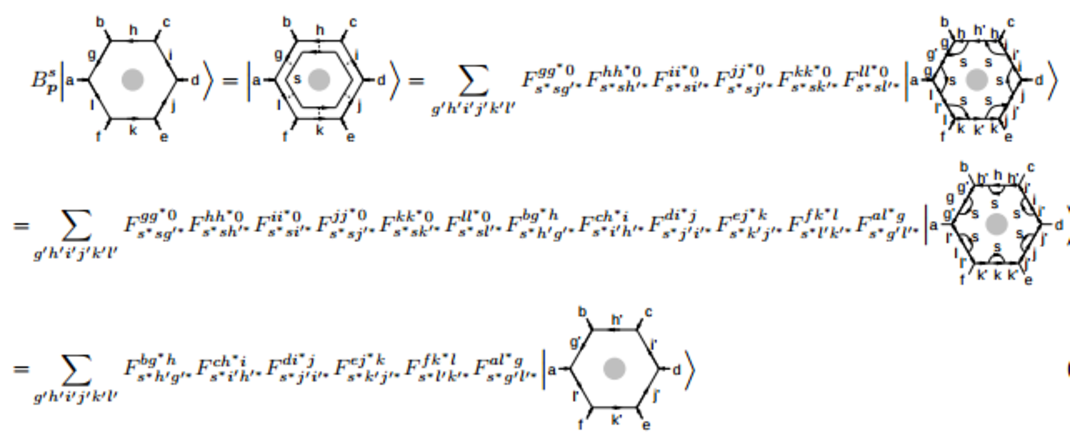
\includegraphics[width=15cm]{B_p_LW.pdf}
\caption[Vertex and Face operators in Levin-Wen model]{Definition of the $Q_{I}$ and $B_{p}$ operators}
\centering
\label{fig:QvBp_Levin_Wen}
\end{figure}
$Q_{I}$ and $B_{p}^{s}$ commute with each other, making the Hamiltonian exactly soluble. The ground state satisfies $Q_{I} = B_{p}^{s} = 1$ for
all $I, p$ while the excited states are those which violate these conditions. 

Given the strings are labelled by UTC $C$, the excitations are given by the monoidal center $Z(C)$ of the UTC $C$, which is a Modular Tensor Category. For example,
consider the Toric code $Z_{2}$, the strings are indexed by one dimensional representations, say, $1$ and $-1$ and the monoidal center of is given by the pair
$(M, \rho)$ where $\rho$ is given by $\rho : \_ \otimes M \rightarrow M \otimes \_ $, which in this case results in a category with rank four, these four form
the excitations in the Toric Code.

\section{Boundary construction, Condensations in String-Net model}

The following work by Kitaev and Kong \citep{Reference4}, presents the relationship between the UTC $C$ and the boundary labels. Consider a lattice with boundary, with edges being labelled
by $M$, which should satisfy all conditions mentioned in the previous section for a valid string-net configuration, that is they should be compatible with the $F$ moves.
Such a structure of the boundary is provided by the left module category over the UTC $C$. Therefore the edge labels on the boundary $M$ are given by the objects of left module category
over the UTC $C$. Given the bulk labels and the boundary labels it is possible to provide the Hamiltonian of the lattice. Once the Hamiltonian is defined, it should be possible 
to compute the ground state, which is used to compute the topological entanglement entropy.

Given the bulk of the lattice is labelled by simple objects from UTC $C$, the excitations are given by the center $Z(C)$ of the UTC $C$, which is a Modular Tensor Category.  
Using the above construction of Modular Tensor Category, the construction of the excitations  on the boundary, the construction of the condensed phase category can be achieved,
as mentioned below. For the detailed proof, refer to \citep{Reference5} \\

Consider the following construction, the excitations of a particular lattice given by UMTC $C$, the boundary excitations by UTC $E$, the condensed phase by another UMTC $D$. 

For one step condesations the following results hold :\\
\begin{itemize}
\item[1] Vacuum of $D$ is given by condensable algebra $A$ in $C$. (condensable implies the algebra is connected, commutative and separable) 
\item[2] $D \simeq C_{A}^{loc}$ category of local right $A$-modules in $C$. 
\item[3] $E \simeq C_{A}$ category of right $A$-modules in $C$. 
\item[4] Anyons in the bulk move onto the wall by the following functor map : 
\begin{center}
  $ \_ \otimes A : C \rightarrow  C_{A}$
\end{center}
\end{itemize}

For two step condensations the following results hold : \\
\begin{itemize}
\item[1] Vacuum in $D$ is given by condensable algebra $A$ in $C$. 
\item[2] $D$ is given by local right A-modules 
\item[3] Vacuum in $E$ is given by connected separable algebra $B$ in $C$. 
\item[4] $E$ is given by $B$-bimodule 
\item[5] Bulk to wall map from the $C$ side is given by :
\begin{center}
  $ \_ \otimes B : C \rightarrow : C_{B|B}$
\end{center}
\end{itemize}

The above statements provide an abstract insight into the relationship between the excitations in the bulk, on the boundary and the condensed phase. Though given the Modular Tensor Category, 
it is not totally possible to construct a lattice model with boundary, as there is no information of the labels in the bulk (the same MTC can be viewed as a center
of different UTC which are equivalent upto Morita equivalence) and also the labels on the boundary. 


% So given $C$, $D$, $E$ how do we find the algebras ! 
% (Indeed this is the one which would give us the boundary objects as well since in both one-step and two step condensations, 
% $E$ is given by right modules of the condensable algebra obtained identified as a vacuum for $D$ (but this reasoning is flawed 
% because we already are given $E$, so there is no need to find $E$. The question is this, given objects in $C'$ whose center 
% $Z(C') = C$, the algebras in $C$ will give us the objects on the boundary $E$ (right modules of the condesable algebras in $C$) 
% So it all boils down to answering the following question, how do we find the algebras in the MTC $C$ ?! \\

% $E$ is given by the Langangrian algebras in $C$.  \\

% For the Double Ising model, $C'$ is given by $1, \sigma, \psi$ and the boundary $E$ is also given by $1, \sigma, \psi$. \\

% The ground state is both the eigen-states of the operators $Q_{v}$ and $B_{p}$, where $Q_{v}$ are fusion rules and $B_{p}$ is given
% by $\varSigma (d_{k}/D^{2}) B_{p}^{k}$, we present the ground states but we do not know how to include excitations (ribbon operators) 
% in these kind of models.

% Construction of ground states on a cylinder with Ising x Ising : \\

% The following satisfy the $Q_{v}$ operator \\
% \begin{center}
% --$v_{1}$------$v_{1}$--\\
%	   $|$\\
%	   $|$\\
%	 $v_{2}$\\
%	   $|$\\
%	   $|$	\\
%--$v_{3}$------$v_{3}$--\\
%\end{center}
%$ (v1, v2, v3) = \{\{1,1,1\} - (1),\{\psi,1,\psi\} - (2),\{\psi,1,1\} - (3),\{\sigma,1,\psi\} - (4), \{\sigma,1,\sigma\} - (5), 
%                   \{\sigma,1,1\} - (6),\{\sigma,\psi,\sigma\} - (7), \{\psi,1,\sigma\} - (8),\{1,1,\sigma\} - (9),\{1,1,\psi\}\ - (10)\}$ \\

%The action of $B_{p}^{1}$ on the above set results in the same set. \\
%The action of $B_{p}^{\psi}$ on the above set results in the following $\{2,1,10,6,5,4,7,9,8,3\}$.\\
%The action of $B_{p}^{\sigma}$ on the above set results in the following 1/sqrt(2) times $\{5+7,5+7,5-7,8+9,1+2+3+10,8+9,1+2-3-10,4+6,4+6,3-7\}$.\\

% Hence we have the following matrices given by $B_p_1, B_p_psi, B_p_sigma$ : \\
%\begin{lstlisting}[frame=single]
%julia> B_p_1 = eye(10);                                                                                                                                                                                                       
%                                                                                                                                                                                                                              
%julia> B_p_psi = [[0 1 0 0 0 0 0 0 0 0]; [1 0 0 0 0 0 0 0 0 0]; [0 0 0 0 0 0 0 0 0 1]; 
%		  [0 0 0 0 0 1 0 0 0 0]; [0 0 0 0 1 0 0 0 0 0]; [0 0 0 1 0 0 0 0 0 0]; 
%		  [0 0 0 0 0 0 1 0 0 0]; [0 0 0 0 0 0 0 0 1 0]; [0 0 0 0 0 0 0 1 0 0]; 
%		  [0 0 1 0 0 0 0 0 0 0]];                                                                                                                                                                                                     
%                                                                                                                                                                                                                              
% julia> B_p_s = [[0 0 0 0 1 0 1 0 0 0]; [0 0 0 0 1 0 1 0 0 0]; [0 0 0 0 1 0 -1 0 0 0]; 
%		[0 0 0 0 0 0 0 1 1 0]; [1 1 1 0 0 0 0 0 0 1]; [0 0 0 0 0 0 0 1 1 0]; 
%		[1 1 -1 0 0 0 0 0 0 -1]; [0 0 0 1 0 1 0 0 0 0]; [0 0 0 1 0 1 0 0 0 0]; 
%		[0 0 0 0 1 0 -1 0 0 0]]                                                                                                                                                                                                   
%
%julia> B_p_sigma = 1/sqrt(2)*B_p_s;                                                                                                                                                                                          
%                                                                                                                                                                                                                              
%julia> B = (1/4)*(B_p_1 + B_p_psi + sqrt(2)*B_p_sigma);                                                                                                                                                                       
%                                                                                                                                                                                                                              
%julia> eigvals(inv(eigvecs(B))*B*eigvecs(B))                                                                                                                                                                                  
%10-element Array{Complex{Float64},1}:                                                                                                                                                                                         
%         -7.91813e-18+0.0im                                                                                                                                                                                                   
%                  1.0+0.0im                                                                                                                                                                                                   
% 8.82083e-18+8.37086e-18im                                                                                                                                                                                                    
% 8.82083e-18-8.37086e-18im                                                                                                                                                                                                    
%                  1.0+0.0im                                                                                                                                                                                                   
%                  1.0+0.0im                                                                                                                                                                                                   
%         -7.14582e-18+0.0im
% 1.27443e-18+1.57887e-18im 
% 1.27443e-18-1.57887e-18im 
%          1.42363e-18+0.0im
 
% julia> eigvecs(inv(eigvecs(B))*B*eigvecs(B))                                                                                                                                                                                  
% 10x10 Array{Complex{Float64},2}:

% \end{lstlisting}

% So for the case of $S_{3}$, the irreps of $D(S_{3})$ form the objects of MTC, while $Rep(S_{3})$ form the objects in UTC. So we need 
% to get the algebras of irreps of $D(S_{3})$ to get the boundaries and once we have the boundaries, we can get the ground state, but then 
% again we need the notion of ribbon operators, which is  missing and Yuting's paper must provide an insight !

\section{Excitations, String operators in String-Net Model}

The excitations in the model are those eigenvectors which do not satisfy the ground state conditions, if $Q_{v} = 0$ is violated the excitation
is a charge excitation at vertex $v$ and is identified by a non-trivial edge label attached to the vertex and if $B_{p}^{s}=0$ is violated 
a fluxon excitation is identified at the plaquette $p$. If all the tail labels are trivial, Levin-Wen lattice is recovered. The lattice with charges are 
invariant under the operators as defined in figure \ref{fig:T1_T4} :
\begin{figure}
\centering
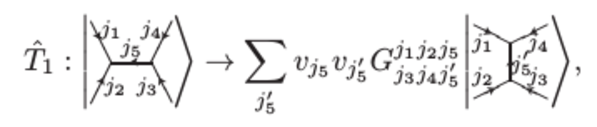
\includegraphics[width=8cm]{T_1_Dyon.pdf}\\
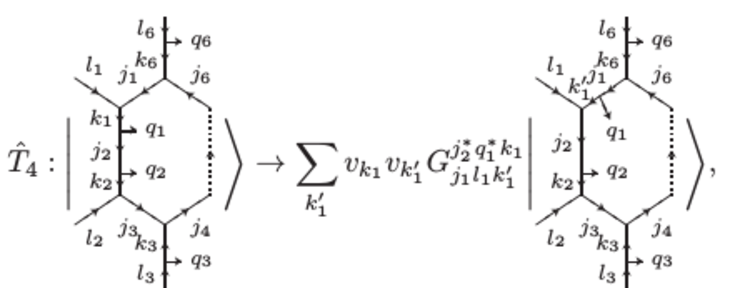
\includegraphics[width=8cm]{T_4_Dyon.pdf}
\caption[Invariant operators in Dyonic model]{Invariant operators in generalized Levin-Wen Model}
\centering
\label{fig:T1_T4}
\end{figure}
The first one is the $F$ move and the second is used to move the non-trivial label around the particular vertex.

The string operator $W_{e}^{J;pq^{*}}$ acting on a state, giving rise to the $J$ fluxon and charges $p$ and $q^{*}$, is as 
given in figure \ref{fig:String_operator}
\begin{figure}
\centering
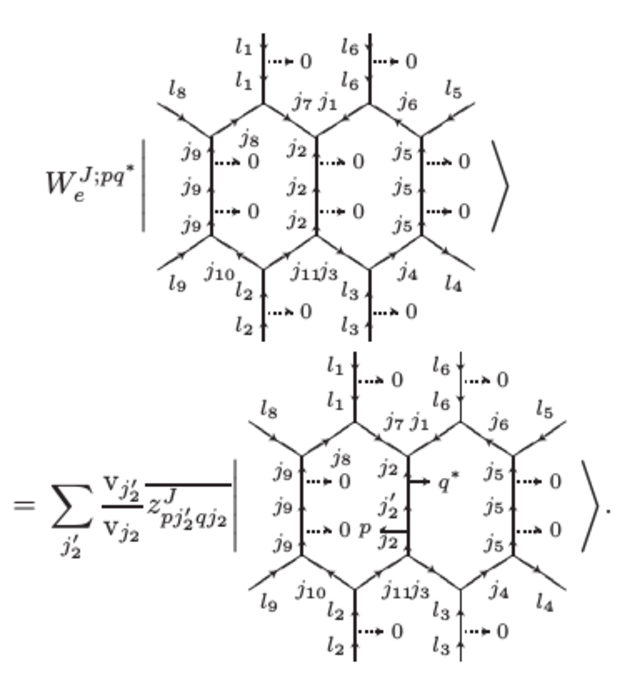
\includegraphics[width=8cm]{String_operator_dyon.pdf}
\caption[String operator in the Dyonic Model]{String operator in generalized Levin-Wen Model}
\centering
\label{fig:String_operator}
\end{figure}

String operator is the ribbon operator equivalent in the String-Net model. For various other operations on the string operators, the charge measurement,
the flux measurement and the action of $Q_{v}^{q}$ and $B_{p}^{s}$ refer to \citep{Reference6}.